\documentclass[12pt]{article}


% Template-specific packages
\usepackage[utf8]{inputenc} % Required for inputting international characters
\usepackage[T1]{fontenc} % Output font encoding for international characters
\usepackage{mathpazo} % Use the Palatino font

\usepackage{graphicx} % Required for including images

\usepackage{booktabs} % Required for better horizontal rules in tables

\usepackage{listings} % Required for insertion of code

\usepackage{enumerate} % To modify the enumerate environment


\title{Parallel Homework \#2}
\author{liukanglai} 
\date{\today}
\usepackage{graphicx}
\graphicspath{{./}}

\usepackage{listings}
\usepackage{xcolor}
\lstset{
    numbers=left,
    numberstyle= \tiny,
    keywordstyle= \color{ blue!70},
    commentstyle= \color{red!50!green!50!blue!50},
    frame=shadowbox, % 阴影效果
    rulesepcolor= \color{ red!20!green!20!blue!20} ,
    escapeinside=``, % 英文分号中可写入中文
    xleftmargin=2em,xrightmargin=2em, aboveskip=1em,
    framexleftmargin=2em
}


\begin{document}

\maketitle

\newpage

\begin{figure}[h]
\centering
\caption{Here is the hardware's information}
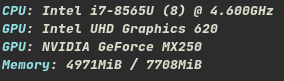
\includegraphics[scale=0.5]{HardwareInfo}
\caption{Here is the cupcores' information}
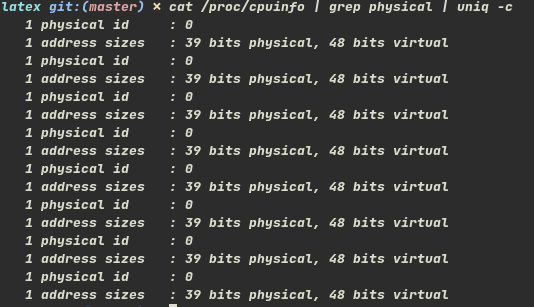
\includegraphics[scale=0.5]{cup_cores}
\caption{Here is the test runing}
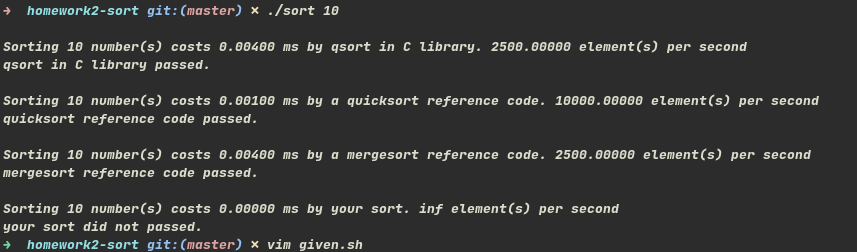
\includegraphics[scale=0.5]{testrunning}
\end{figure}


%echo $(grep -Eo '[0-9\.]+' myfile.txt) >output.txt

I don't know what the meaning of 'under different threads' is...
So I just put the original code and the code using OMP here.

\newpage
\section{running time under different threads}
Sorting 10 number(s) costs 0.00200 ms by qsort in C library. 5000.00000 element(s) per second
qsort in C library passed.

Sorting 10 number(s) costs 0.00100 ms by a quicksort reference code. 10000.00000 element(s) per second
quicksort reference code passed.

Sorting 10 number(s) costs 0.00200 ms by a mergesort reference code. 5000.00000 element(s) per second
mergesort reference code passed.

Sorting 100 number(s) costs 0.01200 ms by qsort in C library. 8333.33333 element(s) per second
qsort in C library passed.

Sorting 100 number(s) costs 0.00500 ms by a quicksort reference code. 20000.00000 element(s) per second
quicksort reference code passed.

Sorting 100 number(s) costs 0.01100 ms by a mergesort reference code. 9090.90909 element(s) per second
mergesort reference code passed.

Sorting 1000 number(s) costs 0.14800 ms by qsort in C library. 6756.75676 element(s) per second
qsort in C library passed.

Sorting 1000 number(s) costs 0.08500 ms by a quicksort reference code. 11764.70588 element(s) per second
quicksort reference code passed.

Sorting 1000 number(s) costs 0.11800 ms by a mergesort reference code. 8474.57627 element(s) per second
mergesort reference code passed.

Sorting 10000 number(s) costs 1.93400 ms by qsort in C library. 5170.63082 element(s) per second
qsort in C library passed.

Sorting 10000 number(s) costs 1.18100 ms by a quicksort reference code. 8467.40051 element(s) per second
quicksort reference code passed.

Sorting 10000 number(s) costs 1.53600 ms by a mergesort reference code. 6510.41667 element(s) per second
mergesort reference code passed.

Sorting 100000 number(s) costs 25.19200 ms by qsort in C library. 3969.51413 element(s) per second
qsort in C library passed.

Sorting 100000 number(s) costs 20.83600 ms by a quicksort reference code. 4799.38568 element(s) per second
quicksort reference code passed.

Sorting 100000 number(s) costs 27.92400 ms by a mergesort reference code. 3581.14883 element(s) per second
mergesort reference code passed.

Sorting 1000000 number(s) costs 177.89700 ms by qsort in C library. 5621.23026 element(s) per second
qsort in C library passed.

Sorting 1000000 number(s) costs 104.67600 ms by a quicksort reference code. 9553.28824 element(s) per second
quicksort reference code passed.

Sorting 1000000 number(s) costs 147.30300 ms by a mergesort reference code. 6788.72800 element(s) per second
mergesort reference code passed.

Sorting 10000000 number(s) costs 1969.10700 ms by qsort in C library. 5078.44419 element(s) per second
qsort in C library passed.

Sorting 10000000 number(s) costs 1158.48200 ms by a quicksort reference code. 8631.98565 element(s) per second
quicksort reference code passed.

Sorting 10000000 number(s) costs 1706.52700 ms by a mergesort reference code. 5859.85455 element(s) per second
mergesort reference code passed.

Sorting 100000000 number(s) costs 22948.90000 ms by qsort in C library. 4357.50733 element(s) per second
qsort in C library passed.

Sorting 100000000 number(s) costs 13038.44200 ms by a quicksort reference code. 7669.62801 element(s) per second
quicksort reference code passed.

Sorting 100000000 number(s) costs 18980.15300 ms by a mergesort reference code. 5268.66143 element(s) per second
mergesort reference code passed.


\textbf{Use OMP:}
Sorting 10 number(s) costs 0.00200 ms by qsort in C library. 5000.00000 element(s) per second
qsort in C library passed.

Sorting 10 number(s) costs 0.00100 ms by a quicksort reference code. 10000.00000 element(s) per second
quicksort reference code passed.

Sorting 10 number(s) costs 0.00200 ms by a mergesort reference code. 5000.00000 element(s) per second
mergesort reference code passed.

Sorting 100 number(s) costs 0.01100 ms by qsort in C library. 9090.90909 element(s) per second
qsort in C library passed.

Sorting 100 number(s) costs 0.00500 ms by a quicksort reference code. 20000.00000 element(s) per second
quicksort reference code passed.

Sorting 100 number(s) costs 0.01000 ms by a mergesort reference code. 10000.00000 element(s) per second
mergesort reference code passed.

Sorting 1000 number(s) costs 0.13900 ms by qsort in C library. 7194.24460 element(s) per second
qsort in C library passed.

Sorting 1000 number(s) costs 0.07400 ms by a quicksort reference code. 13513.51351 element(s) per second
quicksort reference code passed.

Sorting 1000 number(s) costs 0.11200 ms by a mergesort reference code. 8928.57143 element(s) per second
mergesort reference code passed.

Sorting 10000 number(s) costs 1.52100 ms by qsort in C library. 6574.62196 element(s) per second
qsort in C library passed.

Sorting 10000 number(s) costs 1.08100 ms by a quicksort reference code. 9250.69380 element(s) per second
quicksort reference code passed.

Sorting 10000 number(s) costs 1.55800 ms by a mergesort reference code. 6418.48524 element(s) per second
mergesort reference code passed.

Sorting 100000 number(s) costs 28.70700 ms by qsort in C library. 3483.47093 element(s) per second
qsort in C library passed.

Sorting 100000 number(s) costs 19.24300 ms by a quicksort reference code. 5196.69490 element(s) per second
quicksort reference code passed.

Sorting 100000 number(s) costs 25.70000 ms by a mergesort reference code. 3891.05058 element(s) per second
mergesort reference code passed.

Sorting 1000000 number(s) costs 179.66700 ms by qsort in C library. 5565.85238 element(s) per second
qsort in C library passed.

Sorting 1000000 number(s) costs 101.98400 ms by a quicksort reference code. 9805.45968 element(s) per second
quicksort reference code passed.

Sorting 1000000 number(s) costs 143.57000 ms by a mergesort reference code. 6965.24344 element(s) per second
mergesort reference code passed.

Sorting 10000000 number(s) costs 2026.79300 ms by qsort in C library. 4933.90297 element(s) per second
qsort in C library passed.

Sorting 10000000 number(s) costs 1189.48300 ms by a quicksort reference code. 8407.01380 element(s) per second
quicksort reference code passed.

Sorting 10000000 number(s) costs 1619.14400 ms by a mergesort reference code. 6176.10293 element(s) per second
mergesort reference code passed.

Sorting 100000000 number(s) costs 21370.63600 ms by qsort in C library. 4679.31792 element(s) per second
qsort in C library passed.

Sorting 100000000 number(s) costs 12797.54700 ms by a quicksort reference code. 7813.99748 element(s) per second
quicksort reference code passed.

Sorting 100000000 number(s) costs 18511.83500 ms by a mergesort reference code. 5401.94962 element(s) per second
mergesort reference code passed.


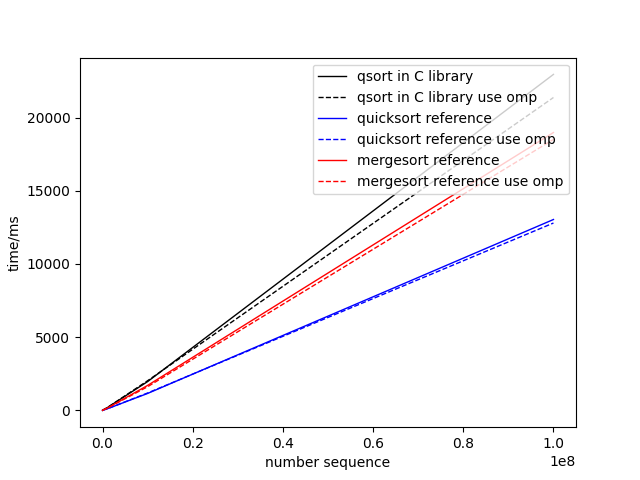
\includegraphics[scale=0.5]{1s}

\section{memory space consumption under different threads}

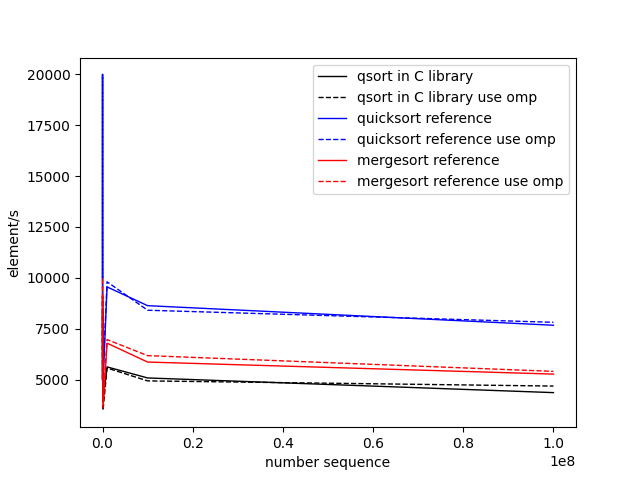
\includegraphics[scale=0.5]{2s}
%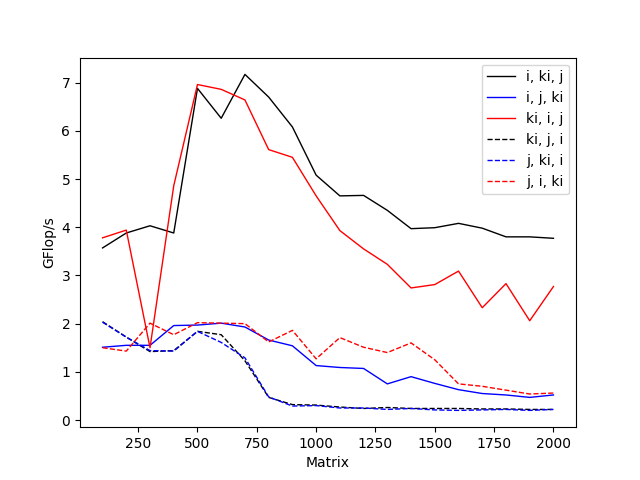
\includegraphics[scale=0.5]{2g}

\section{performance under different input data, using three different input data:}

The following code all use OMP.

\subsection{random number sequence}

Look at 1 and 2.


\subsection{ascending sequence}

The quicksort reference can only run in $10^5$

Sorting 10 number(s) costs 0.41900 ms by a quicksort reference code. 23.86635 element(s) per second, ascending sequence

Sorting 100 number(s) costs 0.50900 ms by a quicksort reference code. 196.46365 element(s) per second, ascending sequence

Sorting 1000 number(s) costs 1.98900 ms by a quicksort reference code. 502.76521 element(s) per second, ascending sequence

Sorting 10000 number(s) costs 131.97800 ms by a quicksort reference code. 75.77020 element(s) per second, ascending sequence

Sorting 100000 number(s) costs 5768.34500 ms by a quicksort reference code. 17.33599 element(s) per second, ascending sequence

Sorting 10 number(s) costs 0.00100 ms by qsort in C library. 10000.00000 element(s) per second, ascending sequence
qsort in C library passed.

Sorting 10 number(s) costs 0.21000 ms by a mergesort reference code. 47.61905 element(s) per second, ascending sequence
mergesort reference code passed.

Sorting 100 number(s) costs 0.00300 ms by qsort in C library. 33333.33333 element(s) per second, ascending sequence
qsort in C library passed.

Sorting 100 number(s) costs 0.69900 ms by a mergesort reference code. 143.06152 element(s) per second, ascending sequence
mergesort reference code passed.

Sorting 1000 number(s) costs 0.03300 ms by qsort in C library. 30303.03030 element(s) per second, ascending sequence
qsort in C library passed.

Sorting 1000 number(s) costs 0.37600 ms by a mergesort reference code. 2659.57447 element(s) per second, ascending sequence
mergesort reference code passed.

Sorting 10000 number(s) costs 0.38200 ms by qsort in C library. 26178.01047 element(s) per second, ascending sequence
qsort in C library passed.

Sorting 10000 number(s) costs 0.56100 ms by a mergesort reference code. 17825.31194 element(s) per second, ascending sequence
mergesort reference code passed.

Sorting 100000 number(s) costs 7.53900 ms by qsort in C library. 13264.35867 element(s) per second, ascending sequence
qsort in C library passed.

Sorting 100000 number(s) costs 3.37400 ms by a mergesort reference code. 29638.41138 element(s) per second, ascending sequence
mergesort reference code passed.

Sorting 1000000 number(s) costs 41.28900 ms by qsort in C library. 24219.52578 element(s) per second, ascending sequence
qsort in C library passed.

Sorting 1000000 number(s) costs 14.83600 ms by a mergesort reference code. 67403.61283 element(s) per second, ascending sequence
mergesort reference code passed.

Sorting 10000000 number(s) costs 437.34700 ms by qsort in C library. 22865.13912 element(s) per second, ascending sequence
qsort in C library passed.

Sorting 10000000 number(s) costs 187.33600 ms by a mergesort reference code. 53380.02306 element(s) per second, ascending sequence
mergesort reference code passed.

Sorting 100000000 number(s) costs 5470.62600 ms by qsort in C library. 18279.44371 element(s) per second, ascending sequence
qsort in C library passed.

Sorting 100000000 number(s) costs 2079.96300 ms by a mergesort reference code. 48077.77831 element(s) per second, ascending sequence
mergesort reference code passed.



\subsection{descending sequence}

Sorting 10 number(s) costs 0.43000 ms by a quicksort reference code. 23.25581 element(s) per second, descending sequence

Sorting 100 number(s) costs 0.47400 ms by a quicksort reference code. 210.97046 element(s) per second, descending sequence

Sorting 1000 number(s) costs 2.72500 ms by a quicksort reference code. 366.97248 element(s) per second, descending sequence

Sorting 10000 number(s) costs 215.21200 ms by a quicksort reference code. 46.46581 element(s) per second, descending sequence

Sorting 100000 number(s) costs 9663.31900 ms by a quicksort reference code. 10.34841 element(s) per second, descending sequence

Sorting 10 number(s) costs 0.00100 ms by qsort in C library. 10000.00000 element(s) per second, descending sequence
qsort in C library did not passed.

Sorting 10 number(s) costs 0.19200 ms by a mergesort reference code. 52.08333 element(s) per second, descending sequence
mergesort reference code passed.

Sorting 100 number(s) costs 0.00400 ms by qsort in C library. 25000.00000 element(s) per second, descending sequence
qsort in C library did not passed.

Sorting 100 number(s) costs 0.21000 ms by a mergesort reference code. 476.19048 element(s) per second, descending sequence
mergesort reference code passed.

Sorting 1000 number(s) costs 0.03300 ms by qsort in C library. 30303.03030 element(s) per second, descending sequence
qsort in C library did not passed.

Sorting 1000 number(s) costs 8.48500 ms by a mergesort reference code. 117.85504 element(s) per second, descending sequence
mergesort reference code passed.

Sorting 10000 number(s) costs 0.45900 ms by qsort in C library. 21786.49237 element(s) per second, descending sequence
qsort in C library did not passed.

Sorting 10000 number(s) costs 2.91500 ms by a mergesort reference code. 3430.53173 element(s) per second, descending sequence
mergesort reference code passed.

Sorting 100000 number(s) costs 8.08400 ms by qsort in C library. 12370.11381 element(s) per second, descending sequence
qsort in C library did not passed.

Sorting 100000 number(s) costs 3.34800 ms by a mergesort reference code. 29868.57826 element(s) per second, descending sequence
mergesort reference code passed.

Sorting 1000000 number(s) costs 38.52800 ms by qsort in C library. 25955.14950 element(s) per second, descending sequence
qsort in C library did not passed.

Sorting 1000000 number(s) costs 13.23200 ms by a mergesort reference code. 75574.36518 element(s) per second, descending sequence
mergesort reference code passed.

Sorting 10000000 number(s) costs 462.86300 ms by qsort in C library. 21604.66488 element(s) per second, descending sequence
qsort in C library did not passed.

Sorting 10000000 number(s) costs 160.67600 ms by a mergesort reference code. 62237.04847 element(s) per second, descending sequence
mergesort reference code passed.

Sorting 100000000 number(s) costs 4802.92300 ms by qsort in C library. 20820.65442 element(s) per second, descending sequence
qsort in C library did not passed.

Sorting 100000000 number(s) costs 1601.46600 ms by a mergesort reference code. 62442.78680 element(s) per second, descending sequence
mergesort reference code passed.


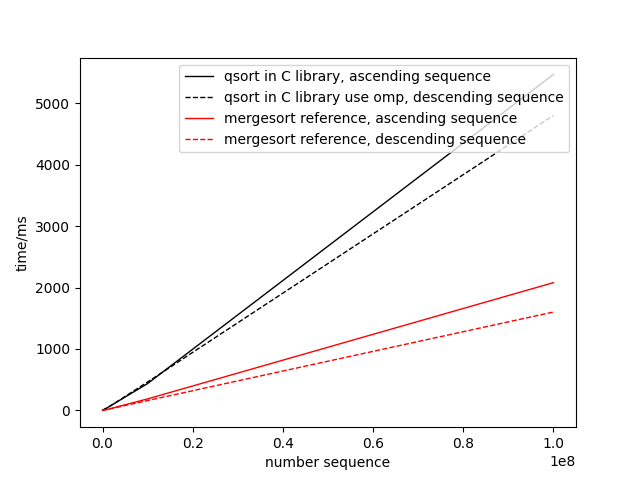
\includegraphics[scale=0.5]{3s}
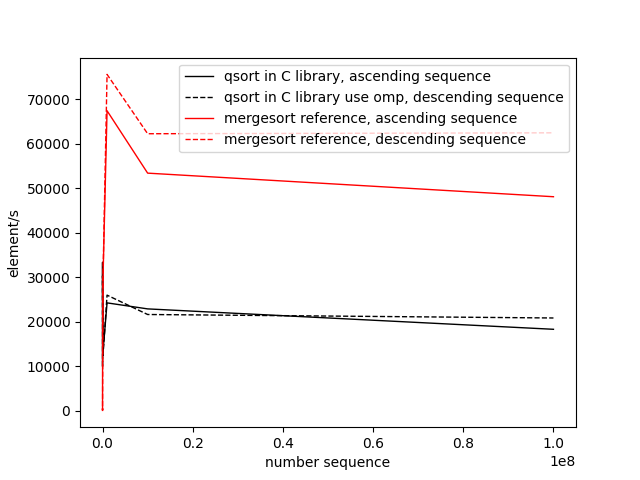
\includegraphics[scale=0.5]{3m}
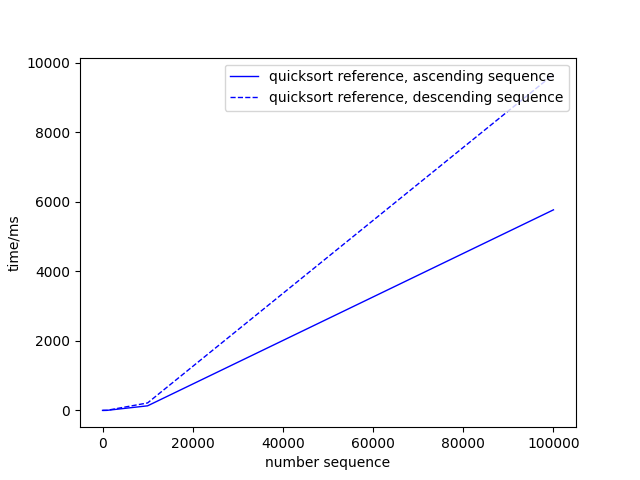
\includegraphics[scale=0.5]{3s1}
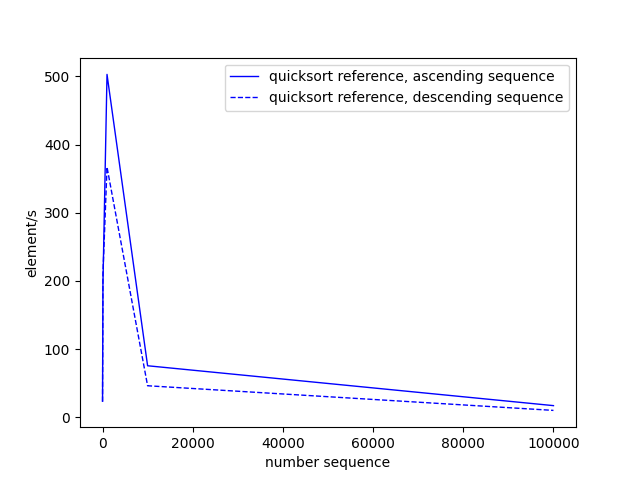
\includegraphics[scale=0.5]{3m1}

The ascending sequence runs slower than the descending sequence firstly, but then it will run faster than that.

\section{performance of qsort () code}

1, 2, 3 all have it, use black color in graphics

%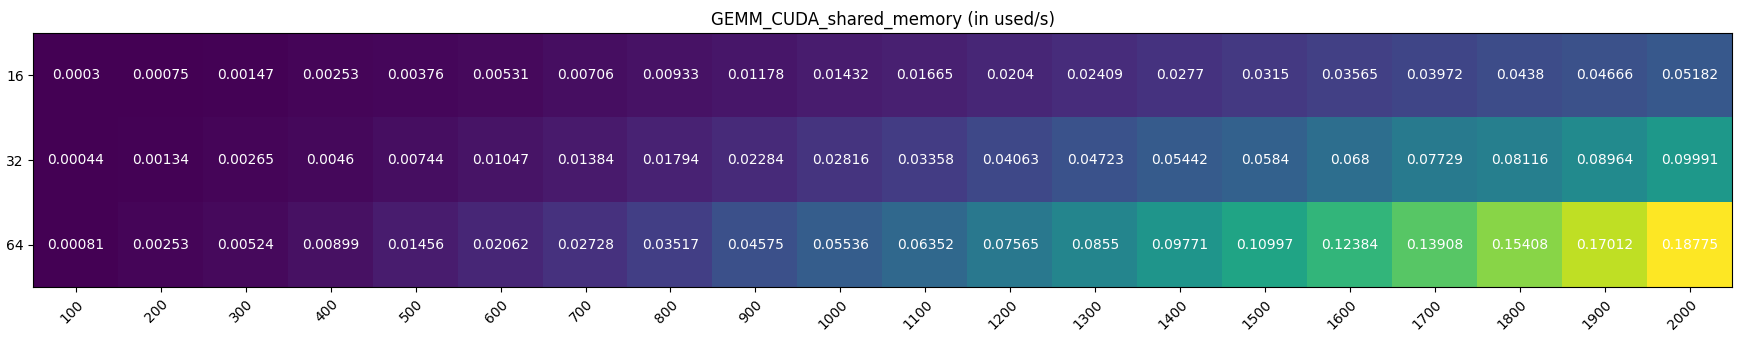
\includegraphics[scale=0.5]{4s}
%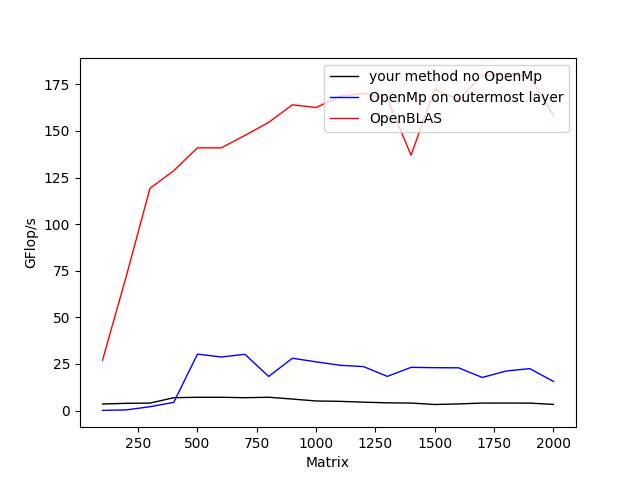
\includegraphics[scale=0.5]{4g}

\section{Original sorting code optimized in any way}

If I have more time, I may find a good sorting code online and to analyse it...
But as I can know, the qsort code in C library is the fastest, just use nlogn time average.


\begin{center}
\Huge{That's all!} \\
\Huge{End!} \\
\end{center} 

\end{document}
